\documentclass{beamer}
\usepackage{parskip}
\usepackage{xcolor}
\usepackage{lipsum}
\usepackage{tikz} 
\usepackage{graphicx}
\usepackage{caption}
\usepackage{animate}
\usepackage{hyperref}
\usepackage{mathrsfs}
\usepackage{amsmath}
\usepackage{amsfonts}

% Set a background template for all slides:
% Load theme: 
\usetheme{ucla}

\colorlet{blockTitleBg}[rgb]{uclaBlueDark}
\colorlet{blockBodyBg}[rgb]{uclaBlue}

\setbeamercolor{block title}{bg=blockTitleBg!80!white, fg=white}
\setbeamercolor{block body}{bg=blockBodyBg!20!white, fg=black}


\usebackgroundtemplate{%
\tikz[overlay,remember picture] \node[opacity=0.1, at=(current page.south east),anchor=south east]{
\includegraphics[height=0.4\paperheight]{bruin_bear.png}};
}

% Set title page values:
\title{Physical Informed Neural Networks}
\date{June 03, 2024}
\author{Lora Yovcheva\\
Mauricio Vargas-Estrada\\
Oscar Iroh\\
Renfei Wang\\
Yilong Liu}

\location{}

% Turn on slide numbers:
\showSlideNumber{}

\begin{document}

\insertTitleSlide

%
% Sample section and sample frame
\section{Section Name}

\begin{frame}{Frame Title}
\framesubtitle{Frame Subtitle} 
    \begin{block}{Block Title}
        Block Content

        \begin{equation}
            u_t + \mathcal{N}(u, \lambda) = 0
        \end{equation}
    \end{block}
\end{frame}

\begin{frame}{Frame Title}
\framesubtitle{Frame Subtitle} 

Unordered list:

\begin{itemize}
    \item Item 1
    \item Item 2
    \item Item 3
\end{itemize}
\end{frame}

\begin{frame}{Frame Title}
\framesubtitle{Frame Subtitle} 

Ordered list:

\begin{enumerate}
    \item Item 1
    \item Item 2
    \item Item 3
\end{enumerate}

\end{frame}
\begin{frame}{Objectives of this study}
\begin{block}{Paper}
        \emph{Raissi, Maziar, Paris Perdikaris, and George E. Karniadakis. 2019. "Physics-informed neural networks: A deep learning framework for solving forward and inverse problems involving nonlinear partial differential equations." Journal of Computational Physics 378: 686-707. https://doi.org/10.1016/j.jcp.2018.10.045}
    \end{block}
\end{frame}

\begin{frame}{Introduction to Physics-Informed Neural Networks}
\begin{block}{}
        \emph{Physics-informed neural networks integrate deep learning with physical laws, enhancing robustness and predictive accuracy.}
    \end{block}
\begin{figure}[H]
    \centering
    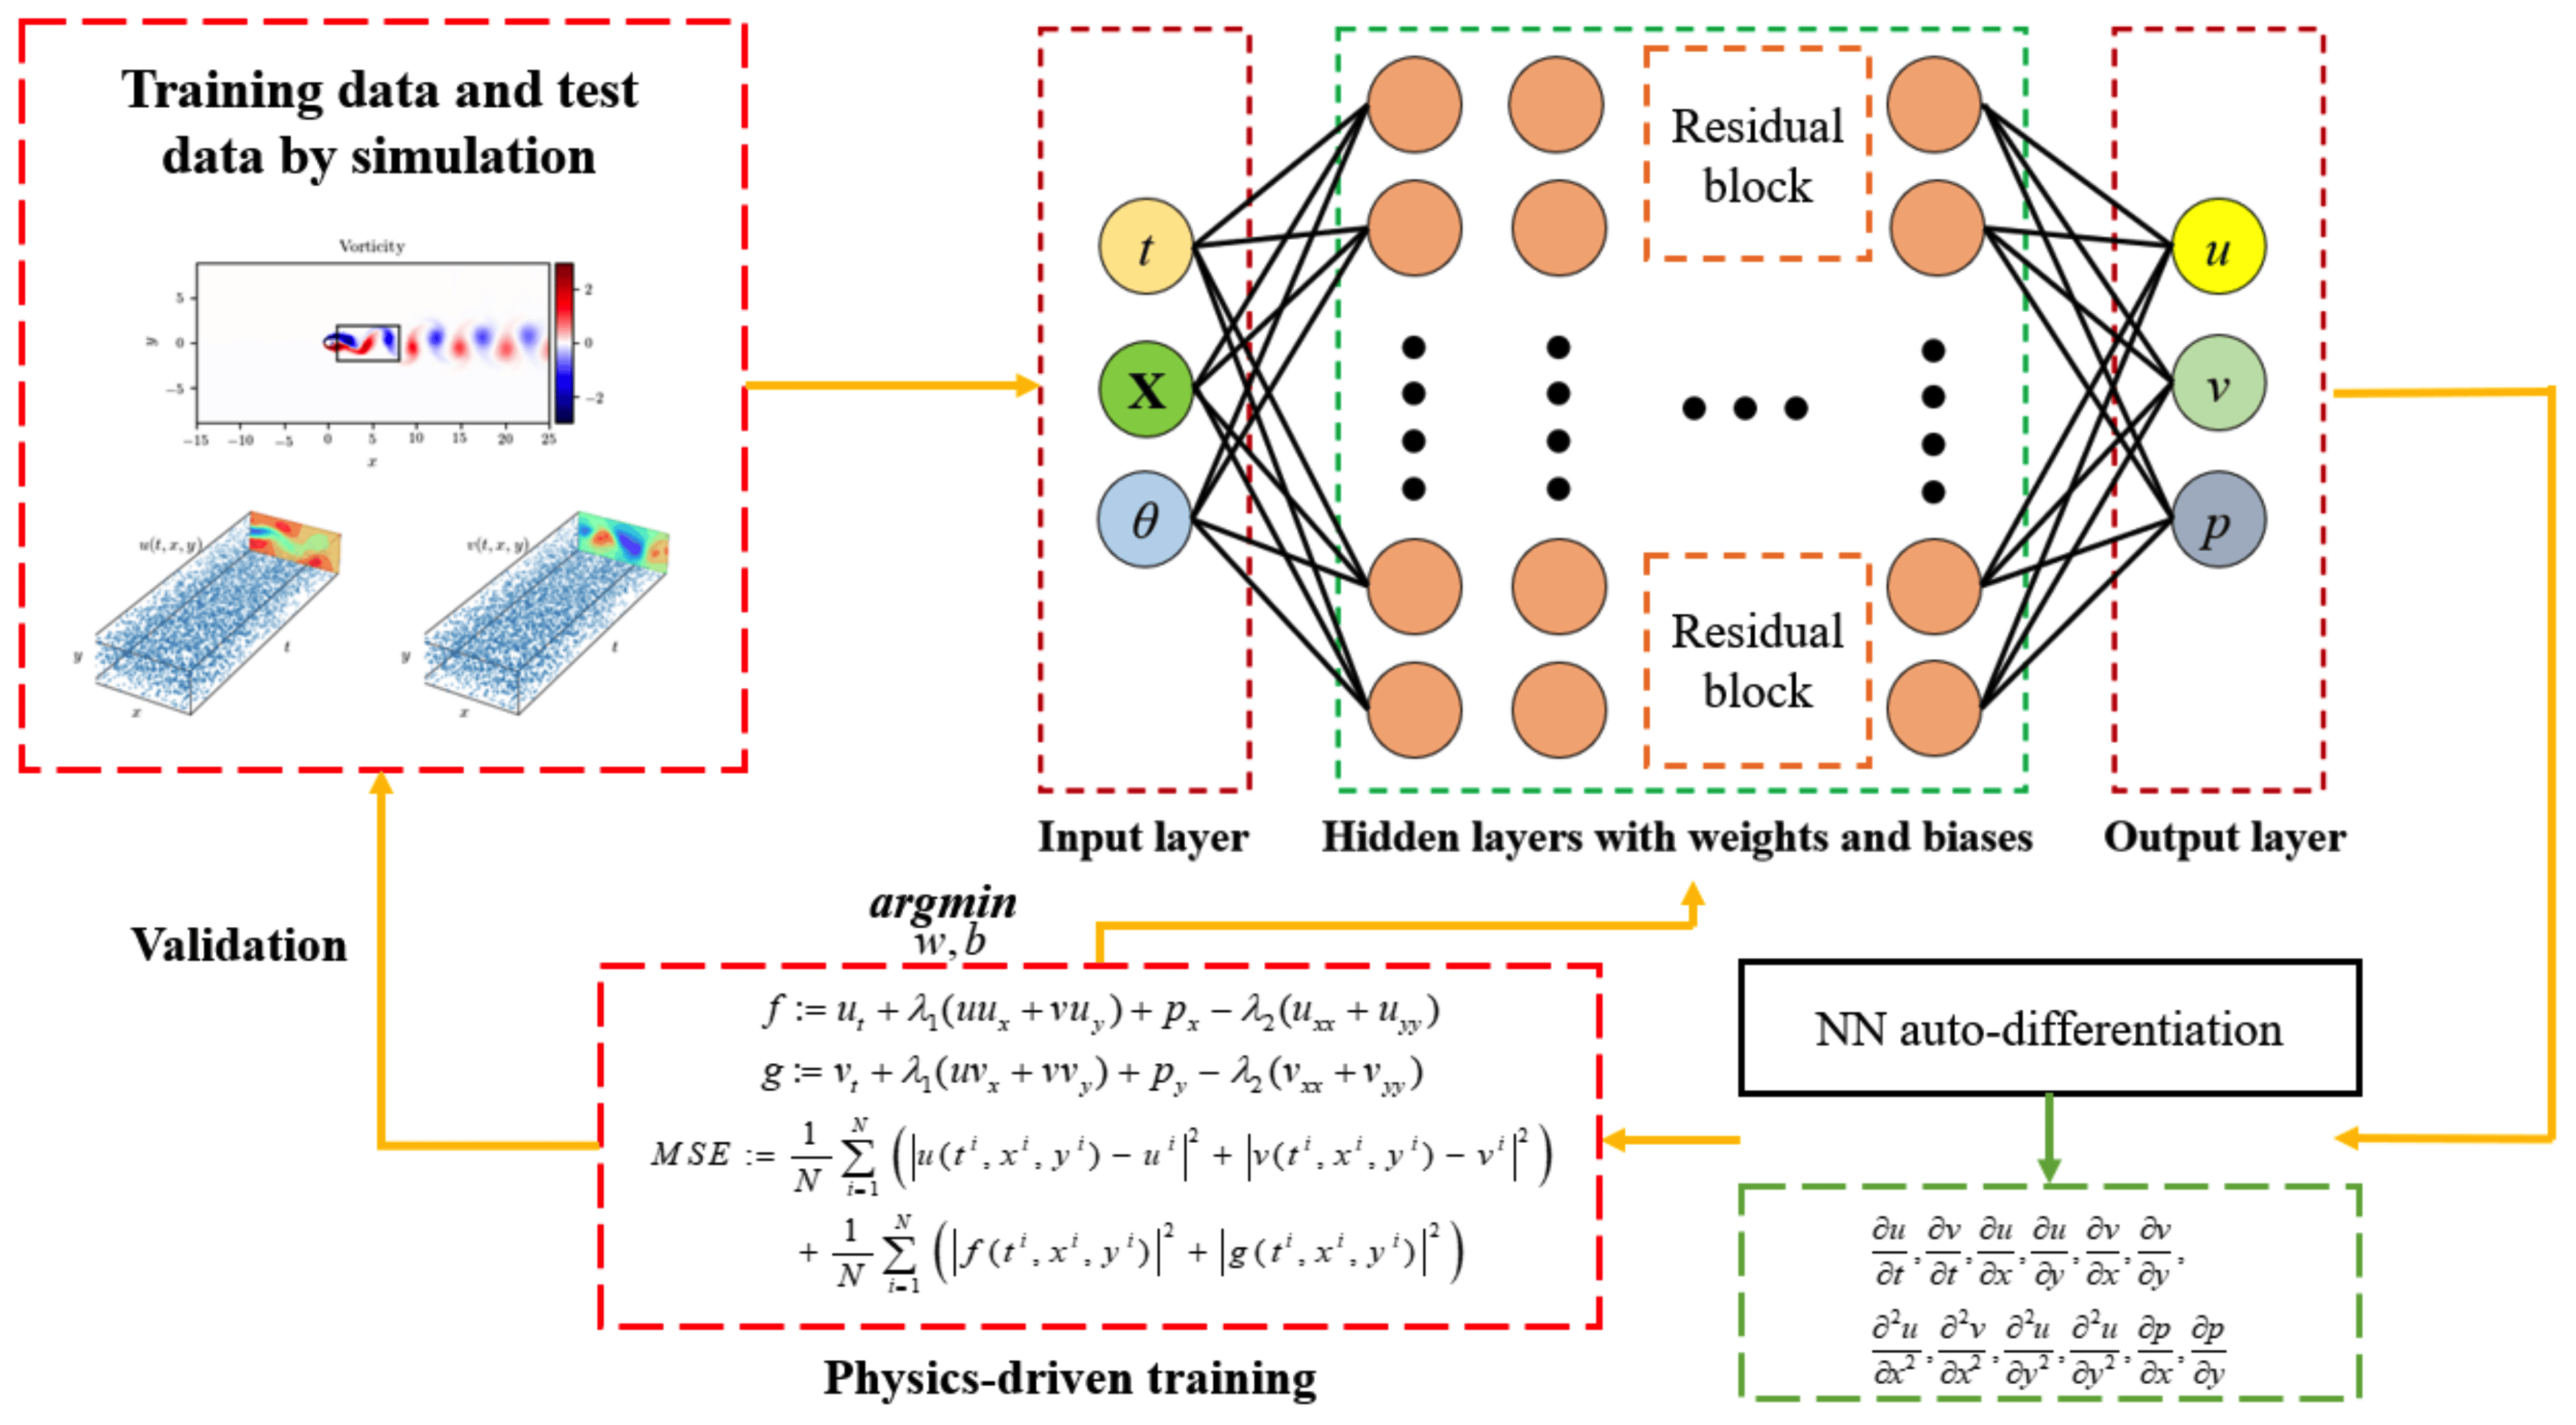
\includegraphics[width=0.8\textwidth]{img/pnn1.png}
    \caption{Schematic of a Physics-Informed Neural Network flow of data.}
    \label{fig:Physics-Informed Neural Networks}
\end{figure} 
\end{frame}

\begin{frame}{Key Components and Insights}
\begin{enumerate}
    \item \textbf{Versatility:} forward and inverse problems in systems described by nonlinear partial differential equations (PDEs)
    \item \textbf{Automatic differentiation (AD):} computation of derivatives up to any order without manual computation. 
    \item \textbf{Deep learning architecture:} facilitates the integration of differential equations directly into the loss function.
    \item \textbf{Computational efficiency:} Leveraging GPU acceleration and efficient training algorithms like L-BFGS (Limited-memory Broyden-Fletcher-Goldfarb-Shanno)
    \item \textbf{Generalizability across domains:} adaptable and can potentially be applied to a wide range of problems (finance, economics, and healthcare)
\end{enumerate}
\end{frame}

\begin{frame}{Theoretical Foundations of PINNs}
General formulation:
\[
u_t + \mathcal{N}[u; \lambda] = 0,
\]
where \( u(t, x) \) is the state variable representing the system's condition at time \( t \) and position \( x \), \( \mathcal{N} \) denotes nonlinear operators reflecting physical dynamics, and \( \lambda \) are parameters influencing these dynamics.
\begin{itemize}
  \item \textbf{Continuous Time Models}: The neural network models function \( u(t, x) \), trained to minimize the residual:
    \[
    f := u_t + \mathcal{N}[u] = 0
    \]
  \item \textbf{Discrete Time Models}: Implement numerical methods like Runge-Kutta for accurate time integration, enhancing model stability and accuracy.
\end{itemize}
\end{frame}

\begin{frame}{Evaluation}
\begin{block}{}
        \emph{Spatio-temporal solution and comparison across specific times.}
    \end{block}
\begin{figure}[H]
    \centering
    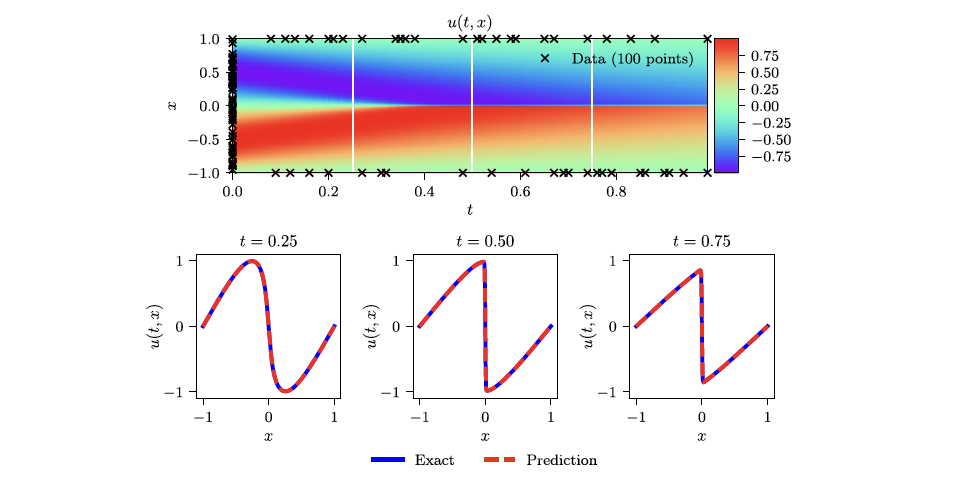
\includegraphics[width=0.8\textwidth]{img/Illustration2.png}
    \caption{Evaluation of PINN Predictions for a Nonlinear PDE.}
    \label{fig:Physics-Informed Neural Networks}
\end{figure} 
\end{frame}

\begin{frame}{Challenges with PINNs}
\begin{enumerate}
    \item \textbf{Sensitivity to hyperparameters:} layers, nodes, learning rates, method of numerical integration. 
    \item \textbf{Numerical stability and convergence:} automatic differentiation can cause problems (like with stochastic gradient descent)
    \item \textbf{Scalability and Computational Demands:} highlights computational intensity in training PINNs, especially with high-dimensional data.
    \item \textbf{Interpretability:} challenges of interpreting deep learning models in econometrics, crucial for understanding variable influences.
\end{enumerate}
\end{frame}

\begin{frame}{Potential Applications}
\textbf{Economics and Econometrics:}
\begin{itemize}
    \item Nonlinear Econometric Modeling
    \item Time Series Analysis
    \item Endogeneity and Instrumental variables
    \item Macroeconomic Modeling
    \item Real-Time Economic Policy Analysis
\end{itemize}
\textbf{Finance:}
\begin{itemize}
    \item Financial Markets
    \item Risk Management and Financial Stress Testing
    \item Portfolio Optimization
\end{itemize}
\end{frame}

\begin{frame}{Relevance to Econometrics}  
PINNs are used in complex econometric systems, particularly in nonlinear dynamics and sparse data scenarios.
\begin{itemize}
    \item \textbf{Model complex dynamics:} irregular data patterns or multi-factor interactions, where traditional models don't work (assumptions of linearity and normality).
    \item \textbf{Improve forecasting accuracy:} deep learning and economic axioms - for macroeconomic indicators and financial markets. 
    \item \textbf{Handle high-dimensional data:} for large numbers of financial instruments or economic indicators. 
    \item \textbf{Robustness for data quality:} reliable predictions in challenging data environments (noise, missing values, or anomalies). 
    \item \textbf{Prior knowledge}: integrate economic theories and constraints directly into the architecture, enhancing the credibility and theoretical consistency of model predictions.
\end{itemize} 
\end{frame}



\begin{frame}{Model}
    \framesubtitle{General form}
        For \( u(x,t) \)
        \begin{equation}
        \text{ s.t. } u_t + \mathcal{N}[u] = 0
        \end{equation}
        Define  
        \begin{equation}
        f := u_t + \mathcal{N}[u]
        \end{equation}
        Then the minimize problem is:
        \begin{equation}
        \min\limits_{u} \text{MSE} = \text{MSE}_u + \text{MSE}_f
        \end{equation}
        where
        \begin{equation}
        \text{MSE}_u = \frac{1}{N_u} \sum_{i=1}^{N_u} | u(t_i^u, x_i^u) - u_i |^2
        \end{equation}
        \begin{equation}
        \text{MSE}_f = \frac{1}{N_f} \sum_{i=1}^{N_f} | f(t_i^f, x_i^f) |^2
        \end{equation}
    \end{frame}
    
    \begin{frame}{Model}
        \begin{block}{Penalty term}
        When we refer to LASSO, the MSE term includes two parts:\\
        the residual and the penalty (which is \( L_1 \) norm of the parameter).\\
        Now, it's actually setting the penalty term as:\\
        \begin{center}
        how far \( f \) is away from 0\\
        \end{center}
        with the physics constraint: 
        \begin{equation}
        f := u_t + \mathcal{N}[u]=0
        \end{equation}
        \end{block}
    \end{frame}
    
    \begin{frame}{Model}
    \framesubtitle{Discrete form and Runge-Kutta method}
        \begin{block}{Runge-Kutta method}
        (Example of a 4-step RK)\\
        Rewrite \( u_t + \mathcal{N}[u] = 0 \) in the form \( u_t = -\mathcal{N}[u] \).\\
        Start with \( u(0, x) = u_0(x) \):
        \begin{enumerate}
            \item Calculate the intermediate values \( k_1, k_2, k_3, k_4 \):
            \begin{align*}
                k_1 &= -\tau \mathcal{N}[u_n], \\
                k_2 &= -\tau \mathcal{N} \left( u_n + \frac{1}{2} k_1 \right), \\
                k_3 &= -\tau \mathcal{N} \left( u_n + \frac{1}{2} k_2 \right), \\
                k_4 &= -\tau \mathcal{N} \left( u_n + k_3 \right).
            \end{align*}
    
            \item Update the solution \( u \) at the next time step:
            \[
            u_{n+1} = u_n + \frac{1}{6} (k_1 + 2k_2 + 2k_3 + k_4).
            \]
        \end{enumerate}
        \end{block}
    \end{frame}
    
    \begin{frame}{Model}
    \framesubtitle{Discrete form and Runge-Kutta method}
        Apply the q-step Runge-Kutta to the general form to create the discrete estimator:
        \begin{equation}
        u_{n+c_i} = u_n - \tau \sum_{j=1}^q a_{ij} \mathcal{N}[u_{n+c_j}], \quad i = 1, \ldots, q
        \end{equation}
        \begin{equation}
        u_{n+1} = u_n - \tau \sum_{j=1}^q b_j \mathcal{N}[u_{n+c_j}]
        \end{equation}
        And the SSE is:
        \begin{equation}
        \text{SSE}_n = \sum_{j=1}^{q+1} \sum_{i=1}^{N_n} \left| u_{n,j}(x_{n,i}) - u_{n,i} \right|^2
        \end{equation}
    \end{frame}    
    
    \begin{frame}{Model}
    \framesubtitle{With boundary on function \( u \) (or multiple equations)}
        The solution of a PDE could change significantly if the equation includes high-order terms.\\
        We may need to add boundary conditions on \( u \) and add another penalty term to the MSE function. That is:
        \begin{equation}
        \mathcal{B}(u) = 0
        \end{equation}
        \begin{equation}
        \text{MSE} = \text{MSE}_u + \text{MSE}_f + \text{MSE}_b
        \end{equation}
        where\\
        \( \mathcal{B}[\cdot] \) is a boundary operator corresponding to Dirichlet, Neumann, Robin, or periodic boundary conditions. 
        \begin{equation}
        \text{MSE}_b = \frac{1}{N_b} \sum_{i=1}^{N_b} | \mathcal{B}(u)(t_i^b, x_i^b) |^2
        \end{equation}
        We could also apply the rule to any other \( u \)-equations.
    \end{frame}
    
    \begin{frame}{Model}
    \framesubtitle{With weight on error}
        The error terms are not necessarily equally weighted.\\
        Given by Raissi, M., Perdikaris, P., Karniadakis, G. E. (2024).\\
        \textit{An Expert’s Guide to Training Physics-informed Neural Networks.}\\
        We could rewrite the MSE function as:
        \begin{equation}
        \text{MSE} = \lambda_u \text{MSE}_u + \lambda_f \text{MSE}_f + \lambda_b \text{MSE}_b
        \end{equation}
    \end{frame}
    
    \begin{frame}{Model}
    \framesubtitle{With weight on error}
        And the \( \lambda \)'s are estimated by:
        \begin{equation}
        \hat{\lambda}_u = \frac{\| \nabla_{\theta} \text{MSE}_u (\theta) \| + \| \nabla_{\theta} \text{MSE}_b (\theta) \| + \| \nabla_{\theta} \text{MSE}_f (\theta) \|}{\| \nabla_{\theta} \text{MSE}_u (\theta) \|}
        \end{equation}
        \begin{equation}
        \hat{\lambda}_f = \frac{\| \nabla_{\theta} \text{MSE}_f (\theta) \| + \| \nabla_{\theta} \text{MSE}_u (\theta) \| + \| \nabla_{\theta} \text{MSE}_b (\theta) \|}{\| \nabla_{\theta} \text{MSE}_f (\theta) \|}
        \end{equation}
        \begin{equation}
        \hat{\lambda}_b = \frac{\| \nabla_{\theta} \text{MSE}_b (\theta) \| + \| \nabla_{\theta} \text{MSE}_f (\theta) \| + \| \nabla_{\theta} \text{MSE}_u (\theta) \|}{\| \nabla_{\theta} \text{MSE}_b (\theta) \|}
        \end{equation}
        where \( \theta \) is the parameter of the network (weights and biases).
    \end{frame}
    
    \begin{frame}{Model}
    \framesubtitle{Estimated result}
        In the Neural Network, we solve the minimize problem of MSE on all potential functions \( u \).\\
        There are two typical ways of using the estimated result.
        \begin{enumerate}
            \item When we do not need the formula of \( u \):\\
            Sometimes we only need the point estimate of the function. It could be either because the analytical solution is hard to solve in a simple form, or because the point estimate is sufficient.
            
            \item When we need the formula of \( u \):
            We should follow the steps to solve for an analytical solution of \( u \):
            \begin{enumerate}
                \item Solve the PDE with function parameters remaining \( u(\gamma) \).
                \item Set an appropriate activation function.
                \item Fit the model to get the estimated \( \hat{u} \).
                \item Estimate the function parameter \( \gamma \) with \( \hat{u} \).
            \end{enumerate}
        \end{enumerate}
    \end{frame}
    
    \begin{frame}{Model}
    \framesubtitle{Prediction failed}
        There are some cases where the prediction may fail:
        \begin{enumerate}
        \item Local minimum.
        \item Convergence difficulty.
        \item Chaotic system.
        \item Physics constraint.   
        \end{enumerate}
        I will list examples for the third and fourth problems.
    \end{frame}
    
    \begin{frame}{Model}
    \framesubtitle{Chaotic system}
        The paper: Steger, S., Rohrhofer, F. M., Geiger, B. C. (2022).\\
        \textit{How PINNs cheat: Predicting chaotic motion of a double pendulum.}\\
        OpenReview shows the predicted result of a double pendulum movement.
        From the graph we could see, for different given conditions at \( t_0 \), the result could be extremely well-fitted or totally unreliable.
        \begin{figure}[H]
            \centering
            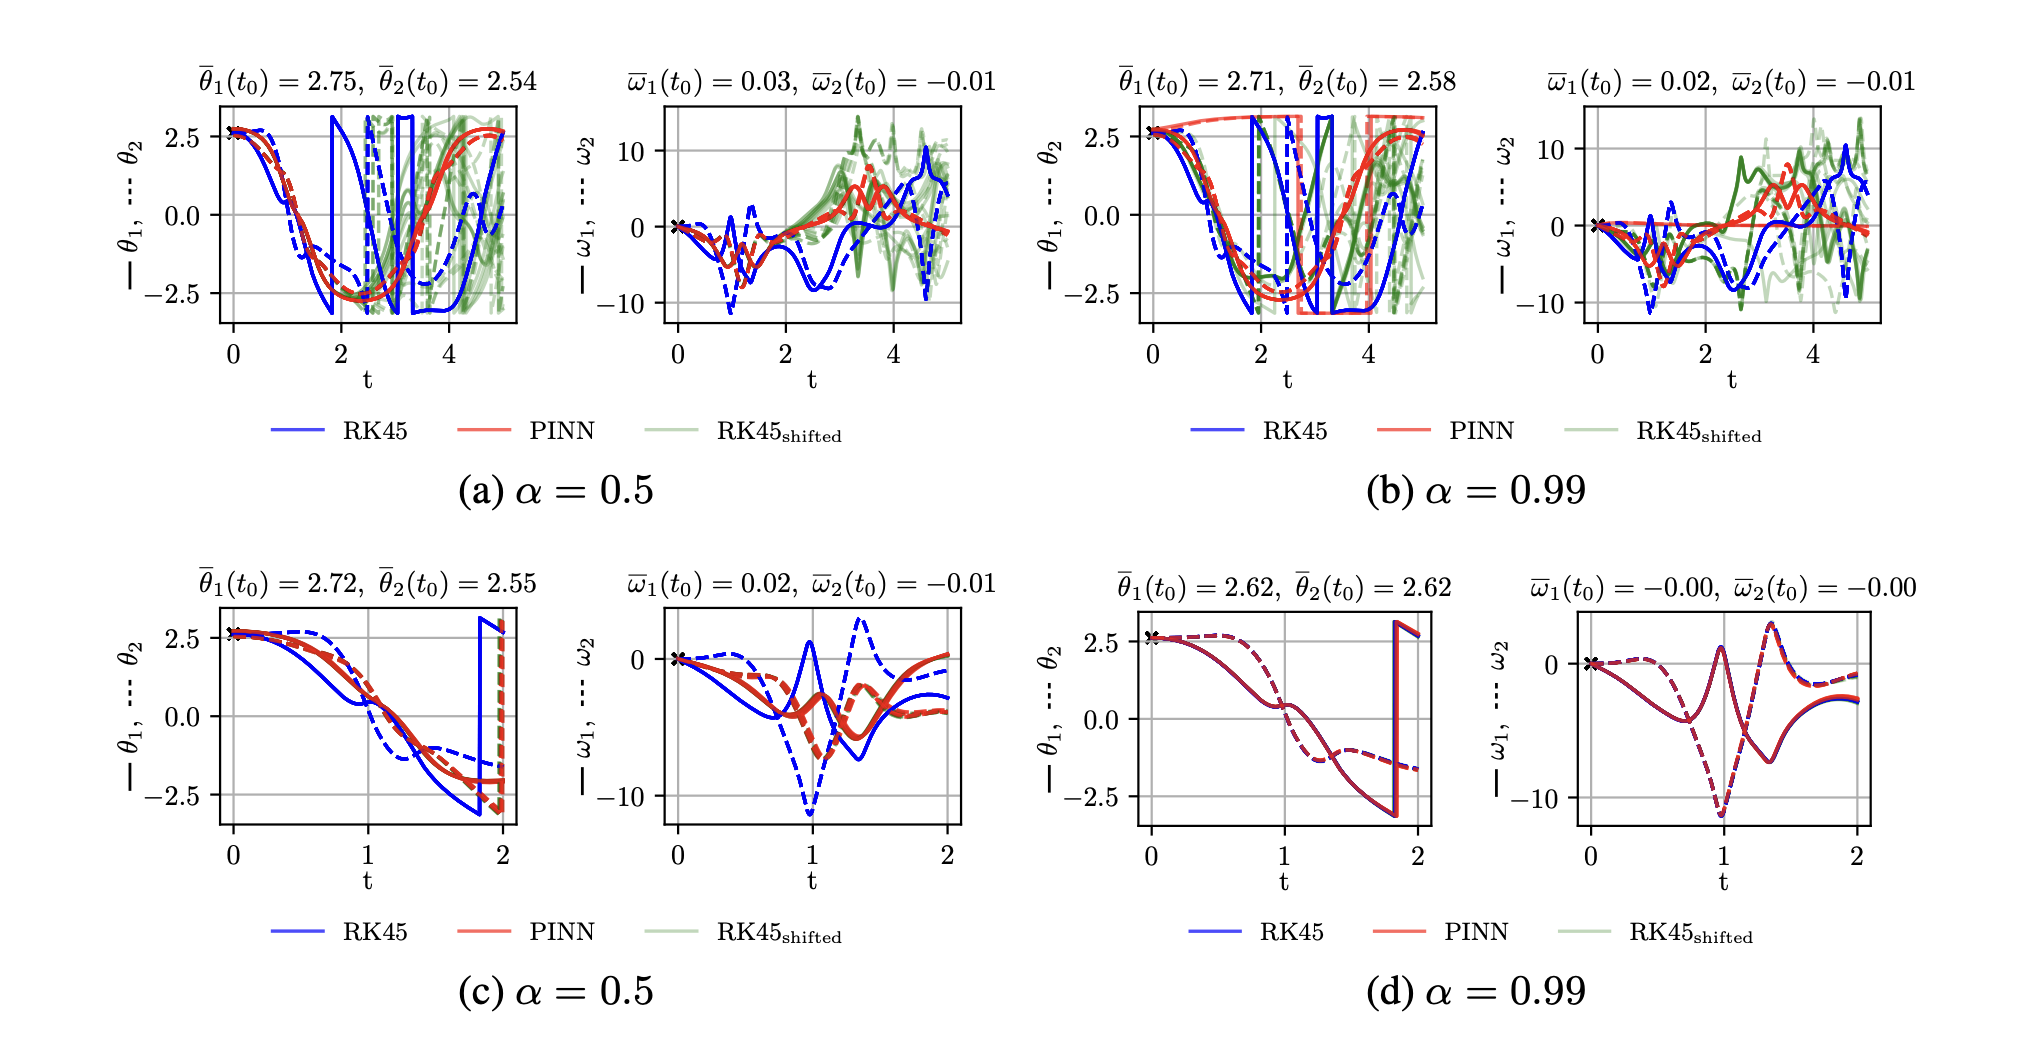
\includegraphics[width=0.8\textwidth]{img/Screenshot 2024-06-02 at 4.02.10 PM}
        \end{figure} 
    \end{frame}
    
    \begin{frame}{Model}
    \framesubtitle{Violate physical causality}
        The paper: Wang, S., Yu, X., Perdikaris, P. (2022).\\
        \textit{Respecting causality is all you need for training physics-informed neural networks.}\\
    
        In the paper, they discovered a convergence difficulty for the problem:
        \begin{equation}
        u_t - 0.0001u_{xx} + 5u^3 - 5u = 0, \quad t \in [0, 1], \quad x \in [-1, 1]
        \end{equation}
        \begin{equation}
        u(x, 0) = x^2 \cos(\pi x)
        \end{equation}
        \begin{equation}
        u(t, -1) = u(t, 1)
        \end{equation}
        \begin{equation}
        u_x(t, -1) = u_x(t, 1)
        \end{equation}
    \end{frame}
    
    \begin{frame}{Model}
    \framesubtitle{Violate physical causality}
        They then found out that because the residual is fitted on each time spot, it cannot capture the temporal causal relationships between physical variables. They adjusted the loss function by adding a weight with a causality parameter:
        \begin{equation}
        \mathcal{L}_r(\theta) = \frac{1}{N_t} \sum_{i=1}^{N_t} w_i \mathcal{L}_r(t_i, \theta)
        \end{equation}
        where
        \begin{equation}
        w_i = \exp \left( -\epsilon \sum_{k=1}^{i-1} \mathcal{L}_r(t_k, \theta) \right)
        \end{equation}
        and \( \epsilon \) is the causality parameter.
    \end{frame}
    
    \begin{frame}{Model}
    \framesubtitle{Violate physical causality: fitting result}
        \begin{figure}[H]
            \centering
            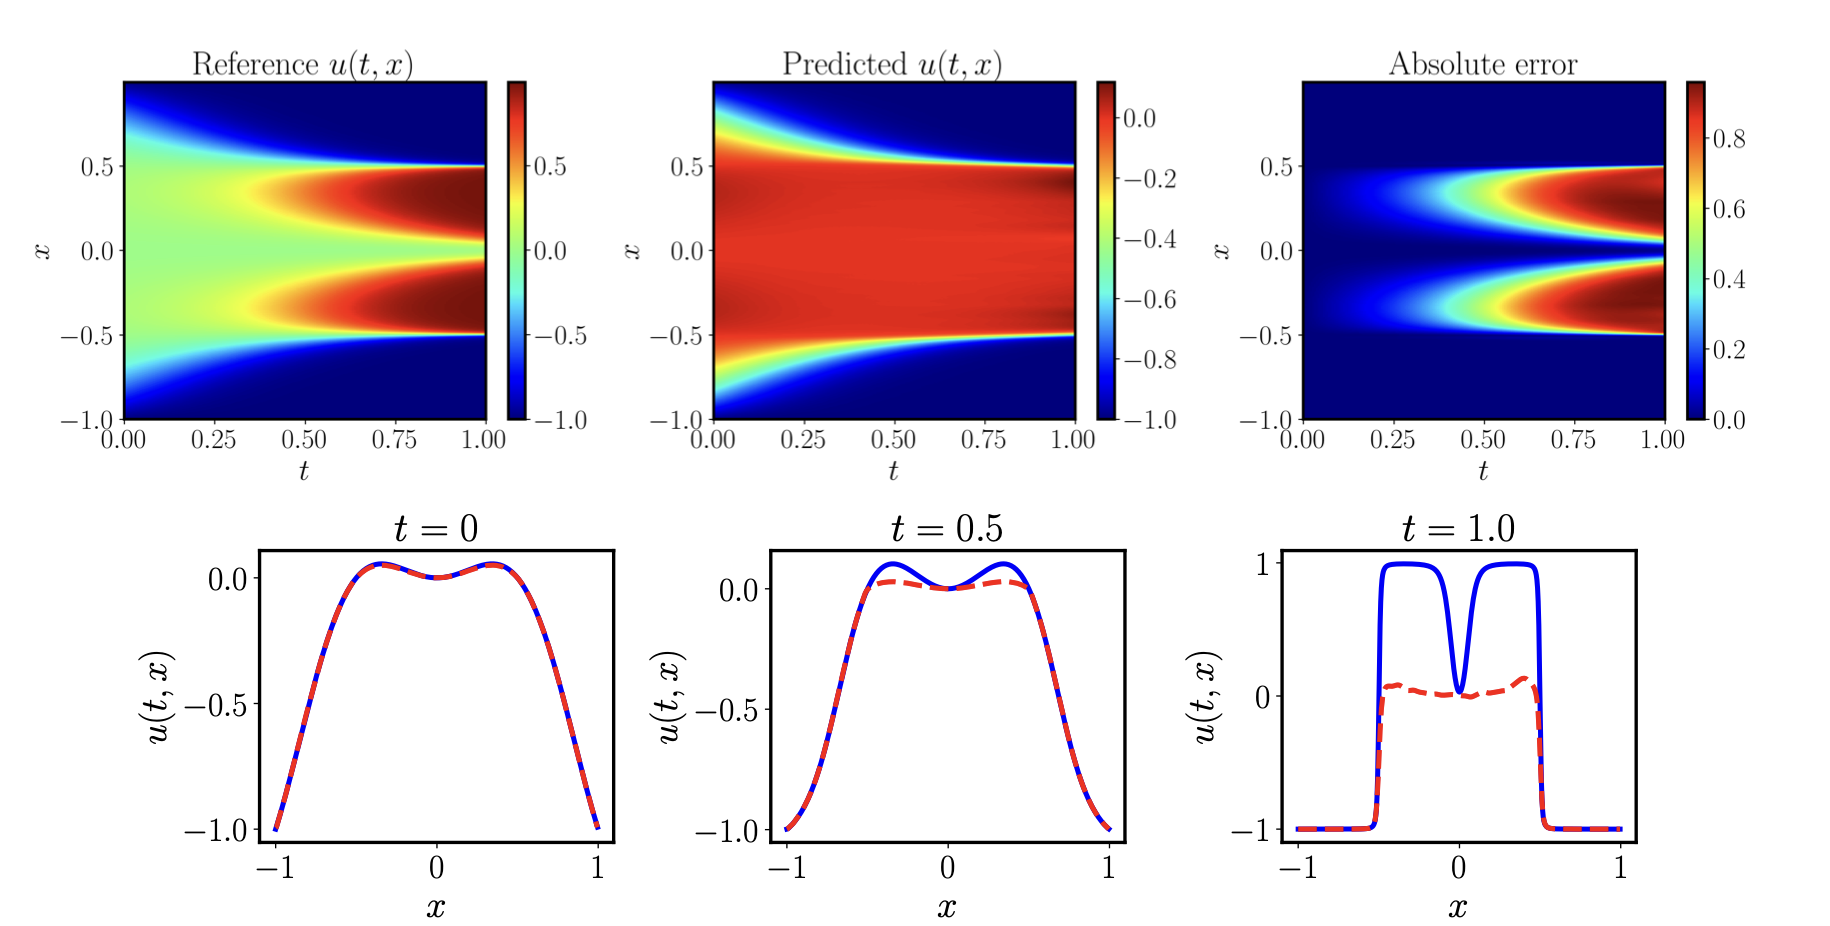
\includegraphics[width=0.55\textwidth]{img/Screenshot 2024-06-02 at 5.03.05 PM}
        \end{figure} 
        \begin{figure}[H]
            \centering
            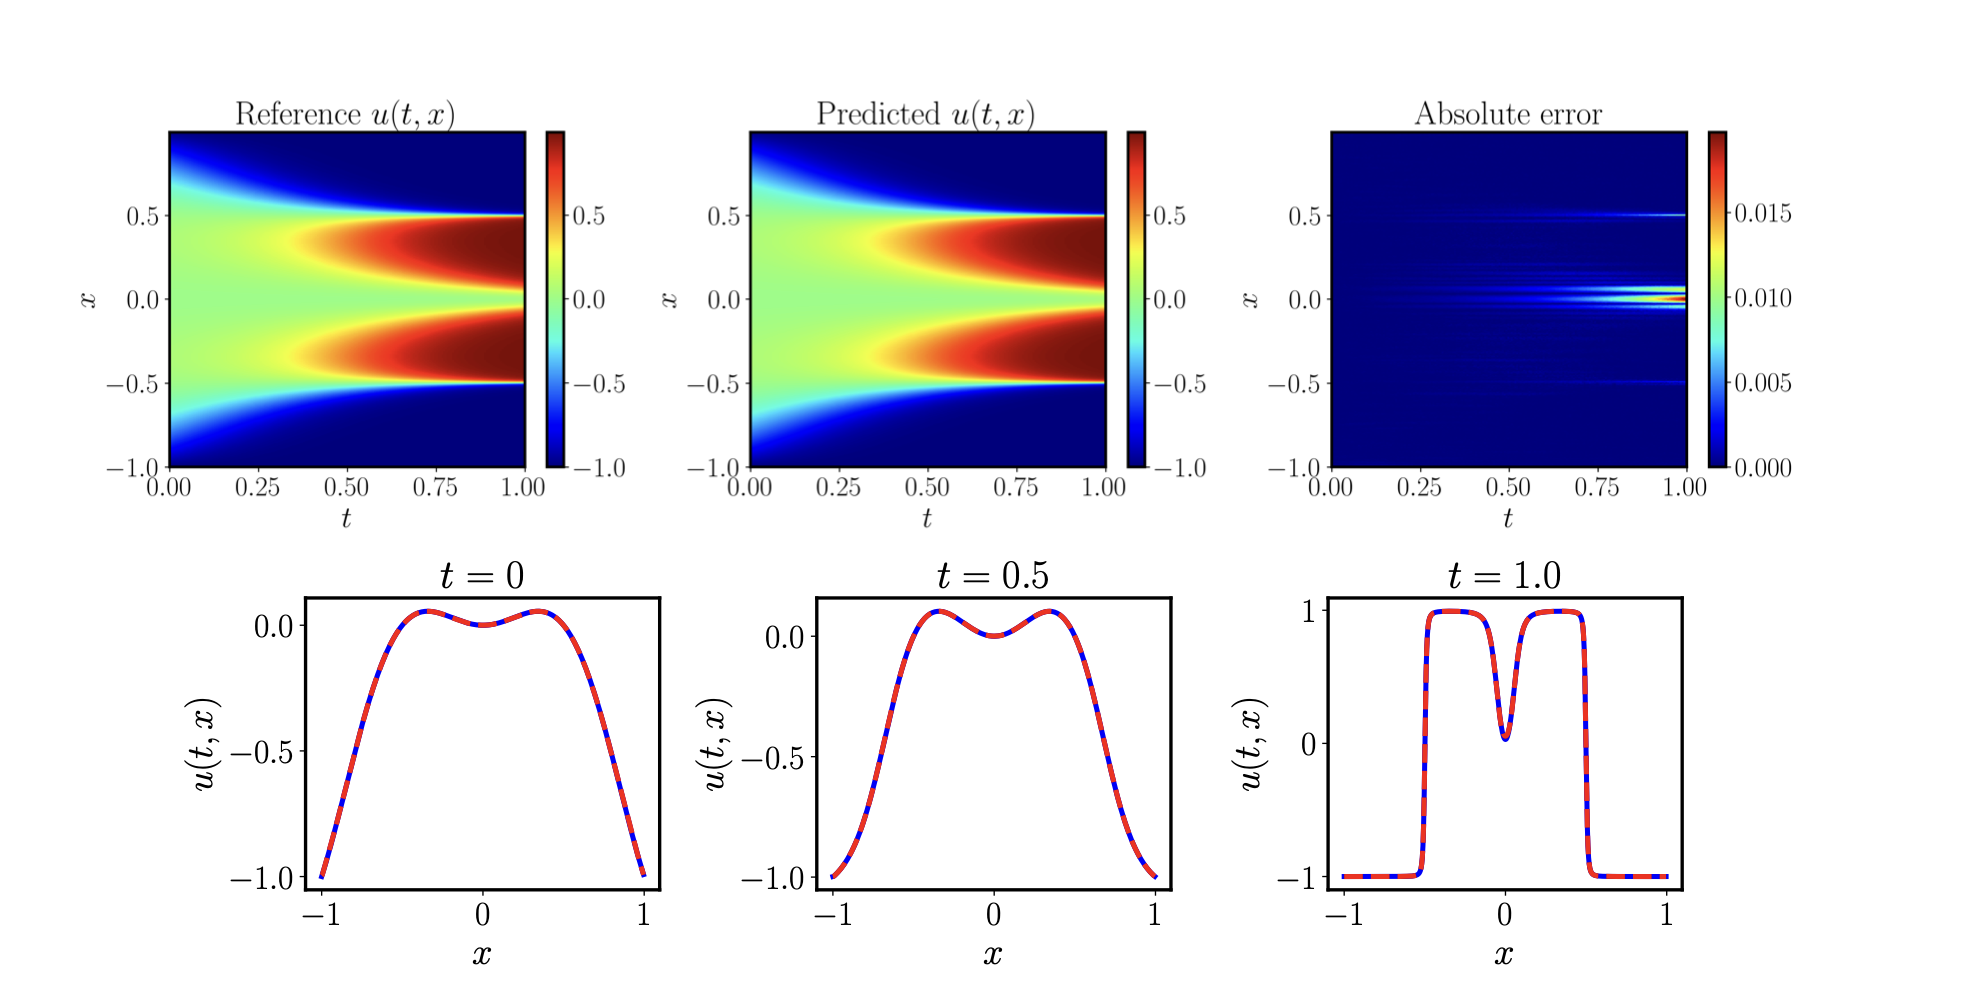
\includegraphics[width=0.6\textwidth]{img/Screenshot 2024-06-02 at 5.03.17 PM}
        \end{figure} 
    \end{frame}
\begin{frame}{Example: Navier-Stokes Equation}

\begin{itemize}
\item Navier-Stokes equations describe the physics of many phenomena of scientific and engineering interest.
\item They may be used to model
    \begin{itemize}
    \item the weather
    \item ocean currents
    \item water flow in a pipe
    \item air flow around a wing. 
    \end{itemize}
\item In their full and simplified forms help with
    \begin{itemize}
    \item the design of aircrafts and cars
    \item the study of blood flow
    \item the design of power stations
    \item the analysis of the dispersion of pollutants
    \end{itemize}
\end{itemize}
\end{frame}

\begin{frame}{Example: Navier-Stokes Equation}
In this example, 
\begin{itemize}
    \item Incompressible flow past a circular cylinder.
    \item Exhibits dynamic behavior and transitions for different Reynolds numbers \( Re = \frac{u_\infty D}{\nu} \).
    \item Parameters: \( u_\infty = 1 \), \( D = 1 \), \( \nu = 0.01 \).
    \item Periodic steady state with asymmetrical vortex shedding.
    \item Known as the Kármán vortex street.
\end{itemize}
\end{frame}

\begin{frame}{Example: Navier-Stokes Equation}
\framesubtitle{Data}
Set of $\{t^i, x^i, y^i, u^i, v^i\}_{i=1}^N$ noisy measures, where:
\begin{itemize}
    \item \( t^i \) is the time of the measurement.
    \item \( x^i \) and \( y^i \) are the spatial coordinates.
    \item \( u^i \) and \( v^i \) are the velocity components in the \( x \) and \( y \) directions, respectively.
\end{itemize}
\end{frame}

\begin{frame}{Example: Navier-Stokes Equation}
\framesubtitle{Data}
Set of $\{t^i, x^i, y^i, u^i, v^i\}_{i=1}^N$ noisy measures, where:
\begin{itemize}
    \item \( t^i \) is the time of the measurement.
    \item \( x^i \) and \( y^i \) are the spatial coordinates.
    \item \( u^i \) and \( v^i \) are the velocity components in the \( x \) and \( y \) directions, respectively.
\end{itemize}

The simulated observations are corrupted with noise. 


The size of the sample is \( N = 5000\), randomly selected from a simulated dataset of  500,000 points in order to show the capacity of the PINN to learn from noisy and scarse data.
\end{frame}

\begin{frame}{Example: Navier-Stokes Equation}
\framesubtitle{Data}
\begin{figure}[H]
    \centering
    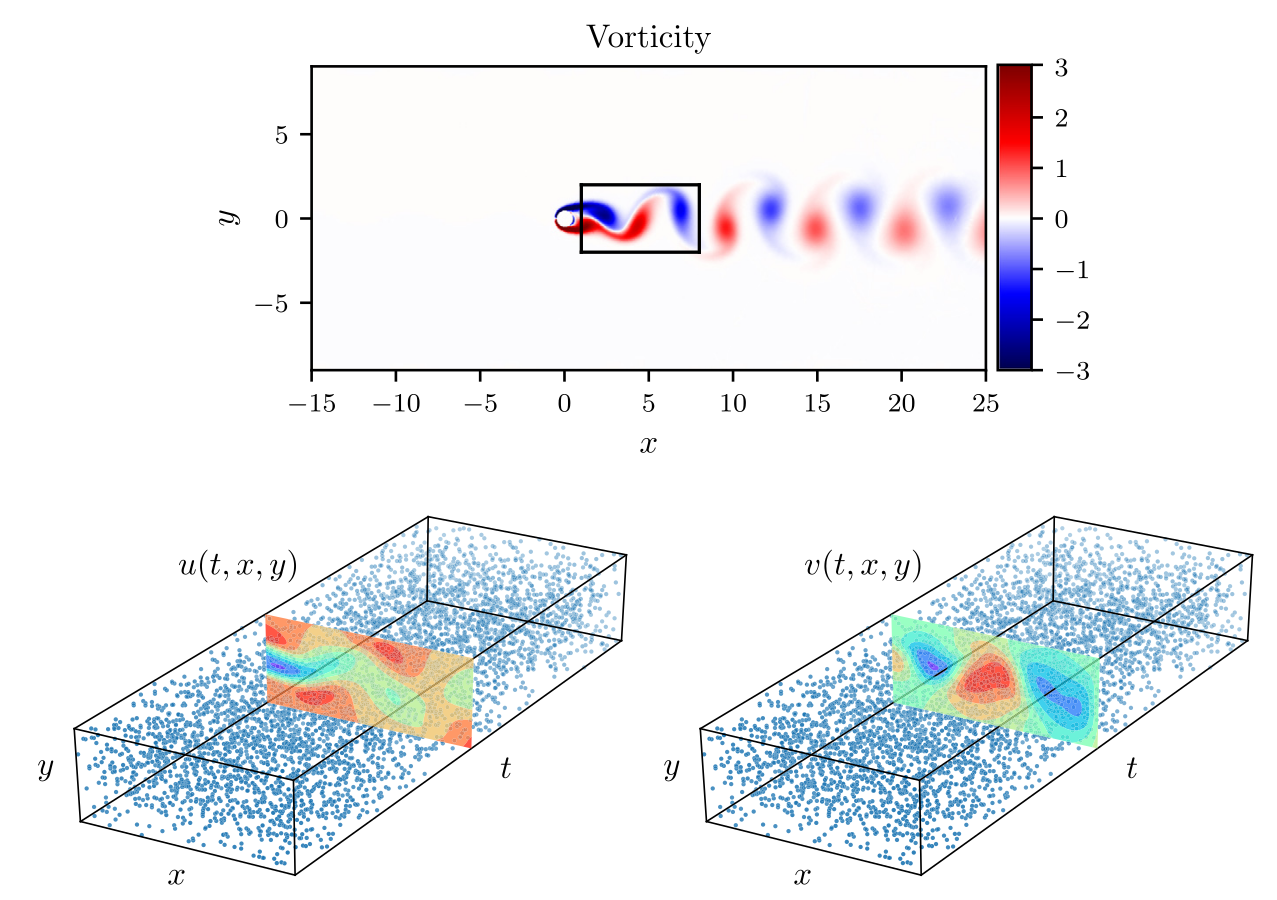
\includegraphics[width=0.8\textwidth]{img/navier-data.png}
\end{figure}
\end{frame}

\begin{frame}{Example: Navier-Stokes Equation}
\framesubtitle{Model}
The explicit form of the Navier-Stokes equations in two dimensions is:
\begin{align}
    u_t + \lambda_1(uu_x + vu_y) = -p_x + \lambda_2(u_{xx} + u_{yy})\\
    v_t + \lambda_1(uv_x + vv_y) = -p_y + \lambda_2(v_{xx} + v_{yy})
\end{align}
where:
\begin{itemize}
    \item $u(t, x, y)$ denotes the $x$-component of the velocity field.
    \item $v(t, x, y)$ denotes the $y$-component of the velocity field.
    \item $p(t, x, y)$ denotes the pressure.
\end{itemize}
Here, $\lambda = (\lambda_1, \lambda_2)$ are the unknown parameters.
\end{frame}

\begin{frame}
An extra equation for the conservation of mass of the fluid is included, 
\begin{align}
    u_x + v_y = 0
\end{align}
where is assumed that
\begin{align}
u = \psi_y \quad \text{and} \quad v = -\psi_x
\end{align}
for some latent function $\psi(t, x, y)$
\end{frame}

\begin{frame}{Example: Navier-Stokes Equation}
\framesubtitle{Architecture}
The neural network architecture is composed of:
\begin{itemize}
    \item input layer with 3 neurons $(t, x, y)$.
    \item 8 hidden layers with 20 neurons each.
    \item output layer with 2 neurons $(u, v)$.
\end{itemize}
\end{frame}

\begin{frame}{Example: Navier-Stokes Equation}
\framesubtitle{Results}
\begin{figure}[H]
    \centering
    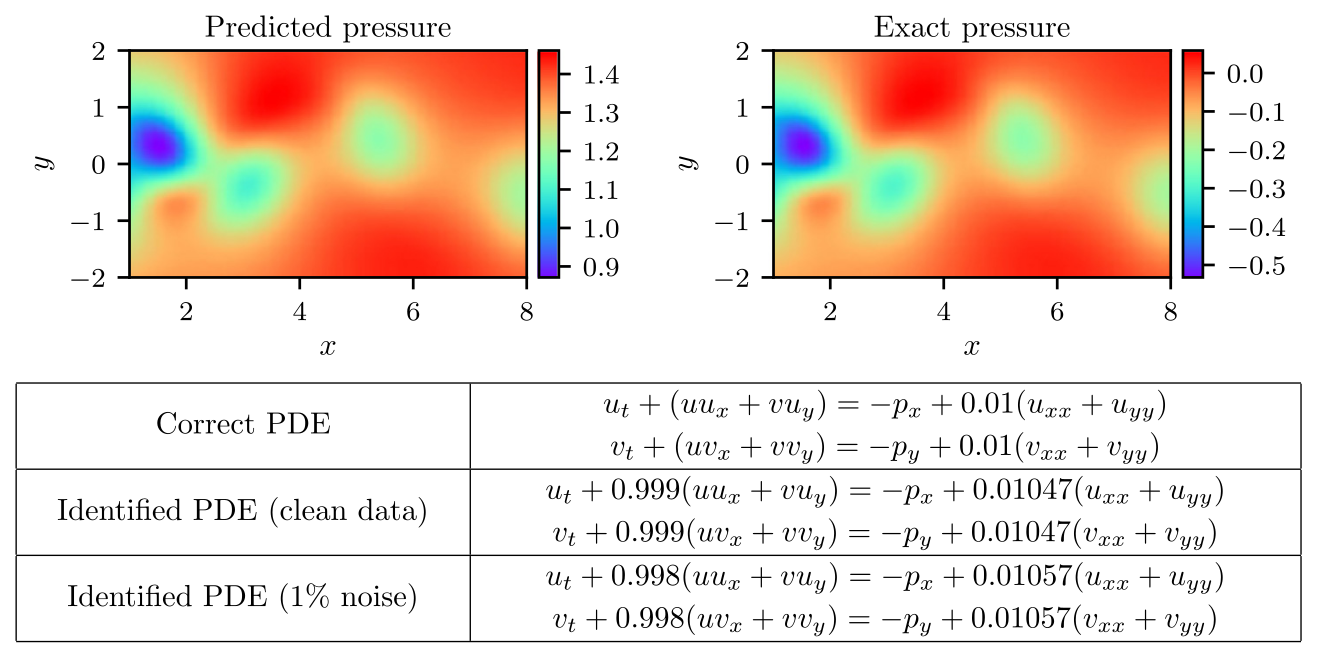
\includegraphics[width=0.8\textwidth]{img/navier-results.png}
\end{figure}
\end{frame}

\begin{frame}{Example: Navier-Stokes Equation}
\framesubtitle{Notes}
The example is fully available in the following repository:
\href{https://github.com/maziarraissi/PINNs}{maziarraisi/PINNs}.

To run the example, instantiate a conda environment with the following dependencies:

\texttt{conda create -n pinn-env python=3.8 tensorflow=1.15 numpy matplotlib scipy}

and activate the environment before running the code:

\texttt{conda activate pinn-env}

\end{frame}
\begin{frame}{Application: PINN in Finance}
    Noguer i Alonso, Miquel and Antolin Camarena, Julian, Physics-Informed Neural Networks (PINNs) in Finance (October 10, 2023). Available at SSRN: \url{https://ssrn.com/abstract=4598180} or \url{http://dx.doi.org/10.2139/ssrn.4598180}
\end{frame}

\begin{frame}{Application: PINN in Finance}
    \begin{block}{Motivation I}
        In the study of finance, Partial Differential Equations (PDEs) and Stochastic Differential Equations (SDEs) are widely applied to model phenomena.  
    \end{block}

    \begin{block}{Motivation II}
        Physics-Informed Neural Networks (PINNs) provide a promising method to solve PDEs by embedding the physical rules into the architecture and training process. 
    \end{block}
\end{frame}

\begin{frame}{Dynamic Systems in Finance}
    \begin{block}{The Black-Scholes Model}
        \begin{equation}
            \frac{\partial V}{\partial t} + \frac{1}{2} \sigma^2 S^2 \frac{\partial^2 V}{\partial S^2} + r S \frac{\partial V}{\partial S} - r V = 0
        \end{equation}
    \end{block}

    \begin{block}{The Physical Part of Loss Function}
        \begin{equation}
            L_{\text{physics}} = \left| \frac{\partial f_{\theta}}{\partial t} + \frac{1}{2} \sigma^2 S^2 \frac{\partial^2 f_{\theta}}{\partial S^2} + r S \frac{\partial f_{\theta}}{\partial S} - r f_{\theta} \right|^2
        \end{equation}
    \end{block}
\end{frame}

\begin{frame}{Dynamic Systems in Finance}
    \begin{block}{The Heston Model}
        \begin{align}
            dS_t &= r S_t \, dt + \sqrt{v_t} S_t \, dW_t^S \\
            dv_t &= \kappa (\theta - v_t) \, dt + \xi \sqrt{v_t} \, dW_t^v
        \end{align}
        where the Feller condition:
        \begin{equation}
            2 \kappa \theta > \xi^2
        \end{equation}
    \end{block}

    \begin{block}{The Physical Part of Loss Function}
        \begin{equation}
            L_{\text{physics}} = \left| \frac{d f_{\theta}^S}{dt} - r f_{\theta}^S - \sqrt{f_{\theta}^v} f_{\theta}^S \right|^2 + \left| \frac{d f_{\theta}^v}{dt} - \kappa (\theta - f_{\theta}^v) - \xi \sqrt{f_{\theta}^v} \right|^2
        \end{equation}
    \end{block}
\end{frame}

\begin{frame}{PINN Approach with The Heston Model}
\framesubtitle{Experiment Set Up}
    \begin{enumerate}
        \item 10,000 trajectories of simulated asset price-volatility pairs.
        \item 252 days.
        \item \(\rho = 0.5\), \(\mu = 0.01\), \(\sigma_S = 2.0\), \(\xi = 0.1\), \(\theta = 0.2\), \(\kappa = 0.075\)
        \item Repeated 100 times
    \end{enumerate}
\end{frame}

\begin{frame}{Experiment Results}
    \begin{figure}[H]
        \centering
        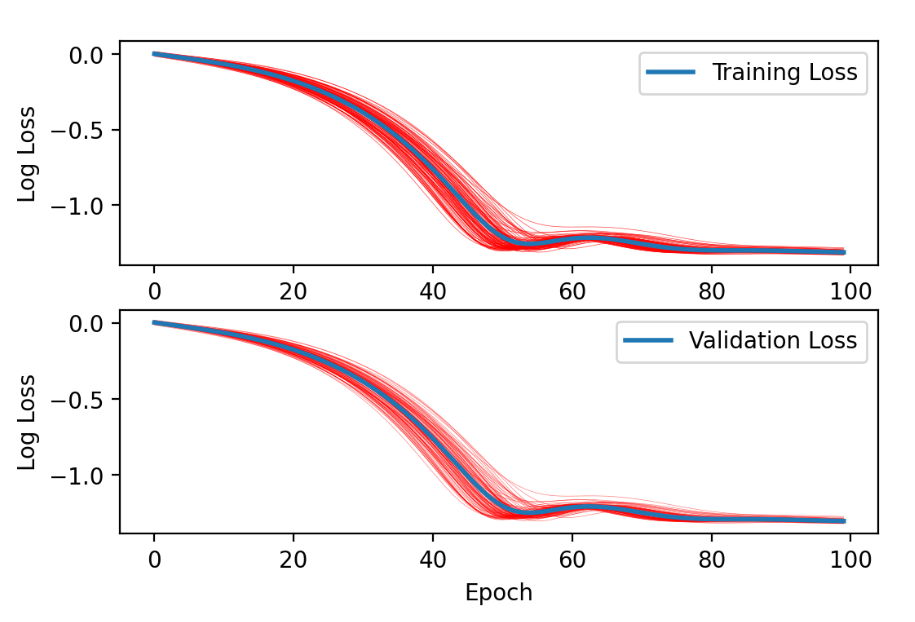
\includegraphics[width=0.8\textwidth]{img/png3.png}
        \caption{Log-loss curves of training and validation losses.}
        \label{fig:log_loss}
    \end{figure}
\end{frame}

\begin{frame}{Experiment Results}
    \begin{figure}[H]
        \centering
        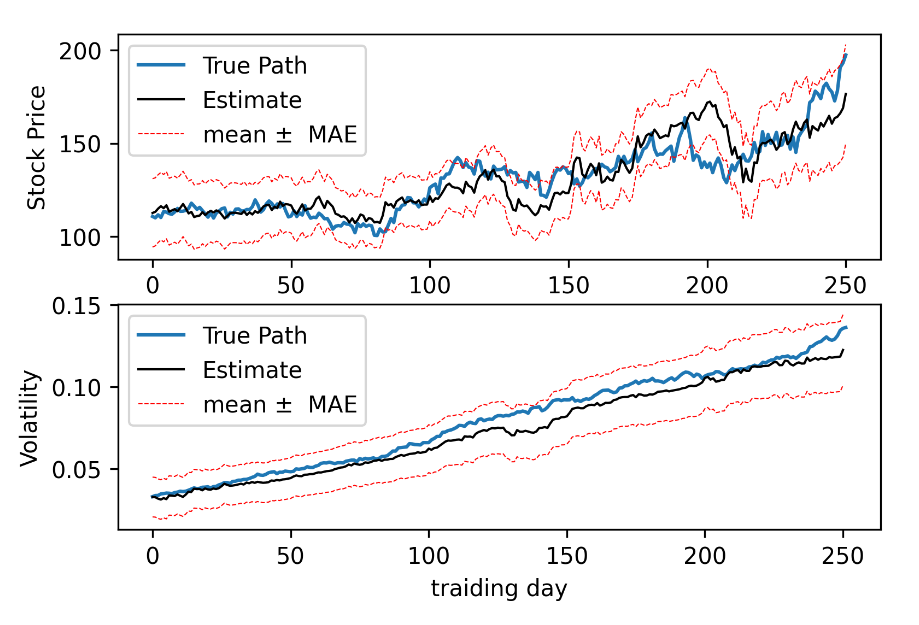
\includegraphics[width=0.6\textwidth]{img/figure2.png}
        \caption{Numerical results of Heston PINN. Top panel: Stock price over a trading year in blue, with the mean PINN prediction in black and the confidence bands at one daily standard deviation. Bottom panel: Volatility of the stock price over a trading year in blue, with the mean PINN prediction in black and the confidence bands at one daily standard deviation.}
        \label{fig:heston_results}
    \end{figure}
\end{frame}

\begin{frame}{Implication and Limitation}
    \begin{enumerate}
        \item PINNs train the Heston model adequately.
        \item The estimated mean is largely within one daily standard deviation of the ground truth, indicating that the Heston model is being learned relatively well.
        \item PINNs not only provide accurate predictions but also ensure that these predictions are consistent with known financial rules and structures. 
        \item The experiment conducted with Heston here is not feasible in reality.
    \end{enumerate}
\end{frame}

\begin{frame}{Implication and Limitation}
    Is it possible to apply this approach to economic studies like macroeconomics?

    Although there is no way to find a parallel universe to test our economic models, we may consider applying this theory to countries whose characteristics converge (for example, OECD countries).

    Xavier X. Sala-i-Martin. (1996). The Classical Approach to Convergence Analysis. The Economic Journal, 106(437), 1019–1036. \url{https://doi.org/10.2307/2235375}
\end{frame}
\begin{frame}{Fitting Procedure}
    Recall the general form of the PDE:
    \begin{equation}
        \frac{\partial u}{\partial t} + \mathcal{N}(u, \lambda) = 0
    \end{equation}

    and 

    \begin{equation}
        f := \frac{\partial u}{\partial t} + \mathcal{N}(u, \lambda)
    \end{equation}

We want to approximate $u(x, t)$ with a neural network $\hat{u}(x, t)$.

For this fitting we required two different sets of data:

\begin{itemize}
    \item Boundary conditions $\mathcal{X}_u$: Points where the solution of the PDE is known.
    \item Corresponding labels $\mathcal{Y}_u$ of the boundary conditions.
    \item Collocation points $\mathcal{X}_f$: Points where the PDE approximation should be valid.
\end{itemize}
\end{frame}

\begin{frame}{Fitting Procedure}
\framesubtitle{Data Sets}

\begin{figure}[H]
    \centering
    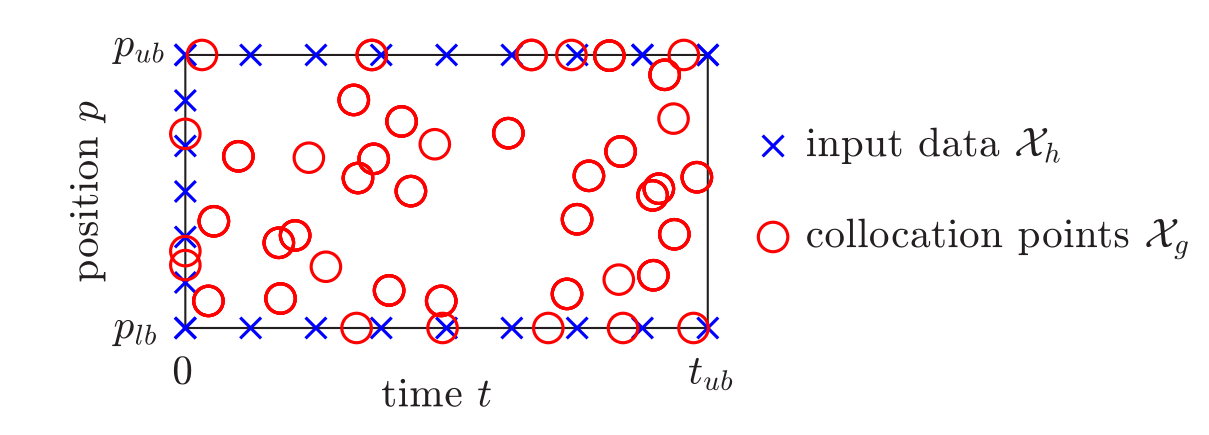
\includegraphics[width=0.8\textwidth]{img/space_time_grid.png}
    \caption{Space-Time grid points of the input data $\mathcal{X}_h$ and $\mathcal{X}_g$}
    \label{fig:space_time_grid}
\end{figure}   

\begin{align}
    \mathcal{X}_u &= \left\{
        \left(x_{u,1}, t_{u,1}\right),
        \cdots,
        \left(x_{u,i}, t_{u,i}\right),
        \cdots,
        \left(x_{u,n_u}, t_{u,n_u}\right)
    \right\}\\
    \mathcal{Y}_u &= \left\{
        u\left(x_{u,1}, t_{u,1}\right),
        \cdots,
        u\left(x_{u,i}, t_{u,i}\right),
        \cdots,
        u\left(x_{u,n_u}, t_{u,n_u}\right)
    \right\}
\end{align}

\begin{equation}
    \mathcal{X}_f = \left\{
        \left(x_{f,1}, t_{f,1}\right),
        \cdots,
        \left(x_{f,i}, t_{f,i}\right),
        \cdots,
        \left(x_{f,n_g}, t_{f,n_f}\right)
    \right\}
\end{equation}
\end{frame}

\begin{frame}{Fitting Procedure}
\framesubtitle{Loss Function}

We divide the loss function in two parts:

\begin{itemize}
    \item Loss function for the boundary conditions:
    \begin{equation}
        \mathcal{L}_u (\mathcal{X}_u, \mathcal{Y}_u, \hat{u}) = \frac{1}{n_u} \sum_{i=1}^{n_u} \left| u(x_{u,i}, t_{u,i}) - \hat{u}(x_{u,i}, t_{u,i})  \right|^2
    \end{equation}
    \item Loss function for the PDE:
    \begin{equation}
        \mathcal{L}_f (\mathcal{X}_f, \hat{u}, \hat{\lambda})= \frac{1}{n_f} \sum_{i=1}^{n_f} \left| \frac{\partial }{\partial t}\hat{u}(x_{f,i}, t_{f, i}) + \mathcal{N}(\hat{u}(x_{f,i}, t_{f, i}), \hat{\lambda}) \right|^2
    \end{equation}
\end{itemize}
\end{frame}

\begin{frame}{Fitting Procedure}
\framesubtitle{Total Loss Function}

The total loss function is given by:

\begin{equation}
    \mathcal{L}(\mathcal{X}_u, \mathcal{Y}_u,\mathcal{X}_f, \hat{u}, \hat{\lambda}) = \mathcal{L}_u (\mathcal{X}_u, \mathcal{Y}_u, \hat{u}) + \mathcal{L}_f (\mathcal{X}_f, \hat{u}, \hat{\lambda})
\end{equation}

And we aim to minimize it with respect to the parameters of the neural network $\hat{u}$ and the parameters of the PDE $\hat{\lambda}$.

\end{frame}
%\begin{frame}{Insight into Challenges \& Future Direction}
 
    \begin{block}{Challenge I: Sensitivity}
    
        One of the primary theoretical challenges is understanding the convergence properties of PINNs. Selecting appropriate hyperparameters is often a trial-and-error process that can be time-consuming and computationally expensive. 

    \end{block}

    \begin{block}{Challenge II: Stability \& Convergence}
    
        The optimization landscape of PINNs is typically non-convex, making it challenging to find global minima.  

    \end{block}
\end{frame}
\begin{frame}
 
    \begin{block}{Challenge III: Scalability and Computational Demands}
    
        PINNs need to be more efficient in handling high-dimensional and multi-scale problems.

    \end{block}

    \begin{block}{Challenge IV: Interpretability}
    
        Real-world data is often noisy and incomplete, which can negatively impact the performance of PINNs. 

    \end{block}
\end{frame}
\begin{frame}{Future Direction}
 
    \begin{block}{High-Dimensional and Multi-Scale Problems}
    
        Addressing the challenges of high-dimensional and multi-scale problems by integrating techniques such as dimensionality reduction, sparse modeling, and hierarchical decomposition. This will broaden the applicability of PINNs to more complex scientific and engineering problems. 

    \end{block}

    \begin{block}{Hybrid Models}
    
        Combining PINNs with traditional numerical methods or other machine learning approaches to leverage the strengths of each. Hybrid models can offer improved accuracy and computational efficiency for solving complex PDEs. 

    \end{block}
\end{frame}
\begin{frame}
 
    \begin{block}{Advancement in Software Tools}
    
        Develop comprehensive software tools and libraries that make it easier for researchers and practitioners to implement, train, and deploy PINNs. These tools should include intuitive interfaces, detailed documentation, and support for various PDEs and boundary conditions.

    \end{block}

    \begin{block}{Transfer Learning and Domain Adaptation}
    
        Tailoring PINNs for specific application domains, such as biomedical engineering, climate modeling, and financial forecasting. This involves incorporating domain-specific knowledge and constraints into the PINN framework.

    \end{block}
\end{frame}
\begin{frame}{Conclusion}
\begin{block}{Long-Term Utility of PINNs}
        \emph{The future direction of PINN research is focused on addressing current challenges, enhancing theoretical understanding, improving computational efficiency, and broadening their applicability through customization and educational initiatives. Given these efforts, PINNs have the potential to revolutionize the way complex differential equations are solved, leading to significant advancements in various scientific and engineering disciplines.}
    \end{block}
\end{frame}

% Insert a last slide to hide backups
\insertLastSlide

\end{document}
